\documentclass[a4paper, 12pt]{article}

%%% SST LAB PROTOCOLL PREAMBLE
%%% 2019
%%%%%%%%%%%%%%%%%%%%%%%%%%%%%%%


%%% PACKAGES
%%%%%%%%%%%%%%%%%%%%%%%%%%%

\usepackage[ngerman]{babel}

\usepackage[utf8]{inputenc}
\usepackage{amsmath}
\usepackage{pgfplots}
\usepackage{tikz}
\usepackage[many]{tcolorbox}
\usepackage{graphicx}
\graphicspath{ {./graphics/} }
\usepackage{pdfpages}
\usepackage{dashrule}
\usepackage{float}
\usepackage{siunitx}
\usepackage{trfsigns}
\usepackage{booktabs}
\usepackage[european]{circuitikz}
\usepackage{tcolorbox}

%%% DOCUMENT GEOMETRY
%%%%%%%%%%%%%%%%%%%%%%%%%%%

\usepackage{geometry}
\geometry{
 a4paper,
 total={0.6180339887498948\paperwidth,0.6180339887498948\paperheight},
 top = 0.1458980337503154\paperheight,
 bottom = 0.1458980337503154\paperheight
 }
\setlength{\jot}{0.013155617496424828\paperheight}
\linespread{1.1458980337503154}

\setlength{\parskip}{0.013155617496424828\paperheight} % paragraph spacing


%%% COLORS
%%%%%%%%%%%%%%%%%%%%%%%%%%%

\definecolor{red1}{HTML}{f38181}
\definecolor{yellow1}{HTML}{fce38a}
\definecolor{green1}{HTML}{95e1d3}
\definecolor{blue1}{HTML}{66bfbf}
\definecolor{hsblue}{HTML}{00b1db}
\definecolor{hsgrey}{HTML}{afafaf}

%%% CONSTANTS
%%%%%%%%%%%%%%%%%%%%%%%%%%%
\newlength{\smallvert}
\setlength{\smallvert}{0.0131556\paperheight}


%%% COMMANDS
%%%%%%%%%%%%%%%%%%%%%%%%%%%

% differential d
\newcommand*\dif{\mathop{}\!\mathrm{d}}

% horizontal line
\newcommand{\holine}[1]{
  	\begin{center}
	  	\noindent{\color{hsgrey}\hdashrule[0ex]{#1}{1pt}{3mm}}\\%[0.0131556\paperheight]
  	\end{center}
}

% mini section
\newcommand{\minisec}[1]{ \noindent\underline{\textit {#1} } \\}

% quick function plot
\newcommand{\plotfun}[3]{
  \vspace{0.021286\paperheight}
  \begin{center}
    \begin{tikzpicture}
      \begin{axis}[
        axis x line=center,
        axis y line=center,
        ]
        \addplot[draw=red1][domain=#2:#3]{#1};
      \end{axis}
    \end{tikzpicture}
  \end{center}
}

% box for notes
\newcommand{\notebox}[1]{

\tcbset{colback=white,colframe=green1!100!black,title=Note!,width=0.618\paperwidth,arc=0pt}

 \begin{center}
  \begin{tcolorbox}[]
   #1 
  \end{tcolorbox}
 
 \end{center} 
 
}

% box for equation
\newcommand{\eqbox}[2]{
	
	\tcbset{colback=white,colframe=green1!100!black,title=,width=#2,arc=0pt}
	
	\begin{center}
		\begin{tcolorbox}[ams align*]
				#1
		\end{tcolorbox}
		
	\end{center} 
	
}
% END OF PREAMBLE

%%%%%%%%%%%%%%%%%%%%%%%%%%%%%%%%%%%%%

\begin{document}

%%%%%%%%%%%%%%%%%%%%%%%%%%%%%%%%%%%%%
  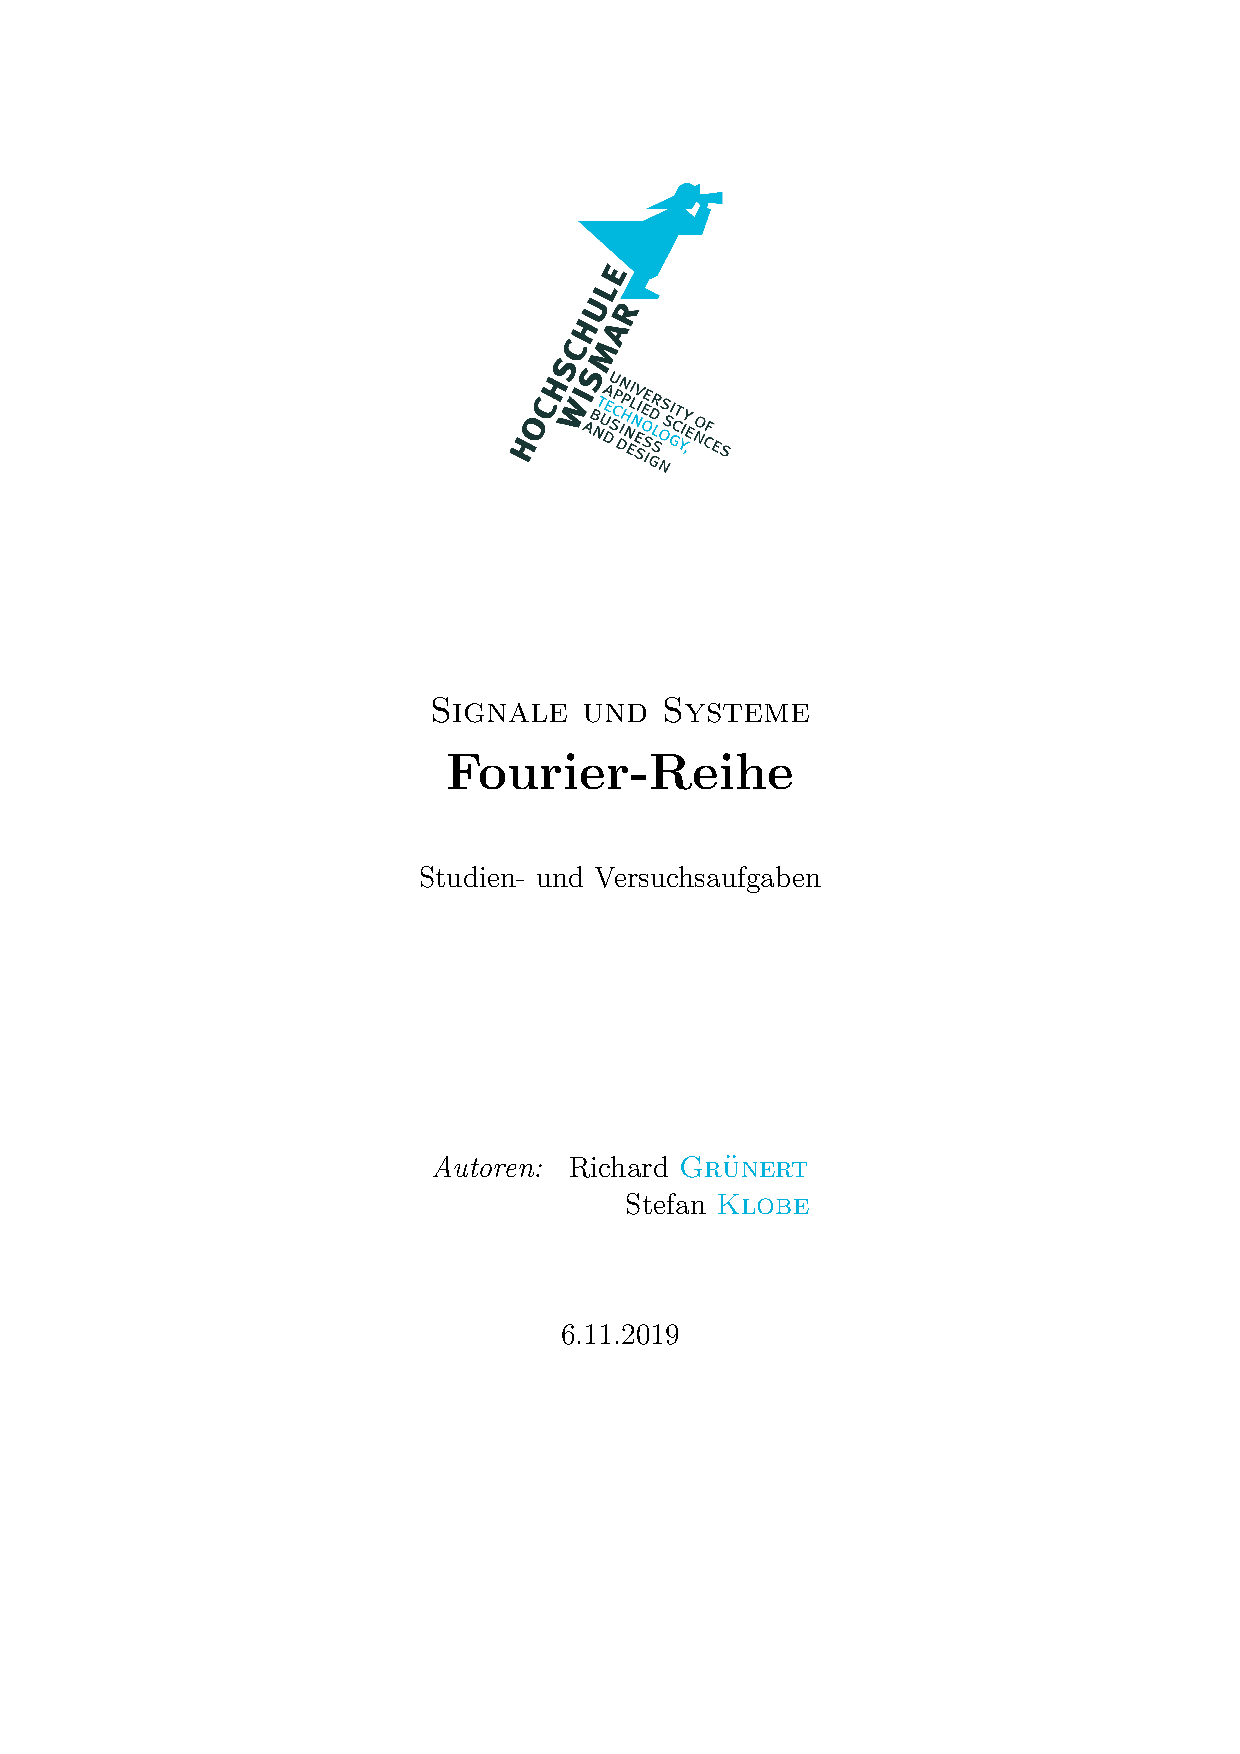
\includepdf{./titlepage/titlepage.pdf}
  \clearpage
  \setcounter{page}{1}
%%%%%%%%%%%%%%%%%%%%%%%%%%%%%%%%%%%%%

\section{Vorbereitungsaufgaben}


\subsection{}
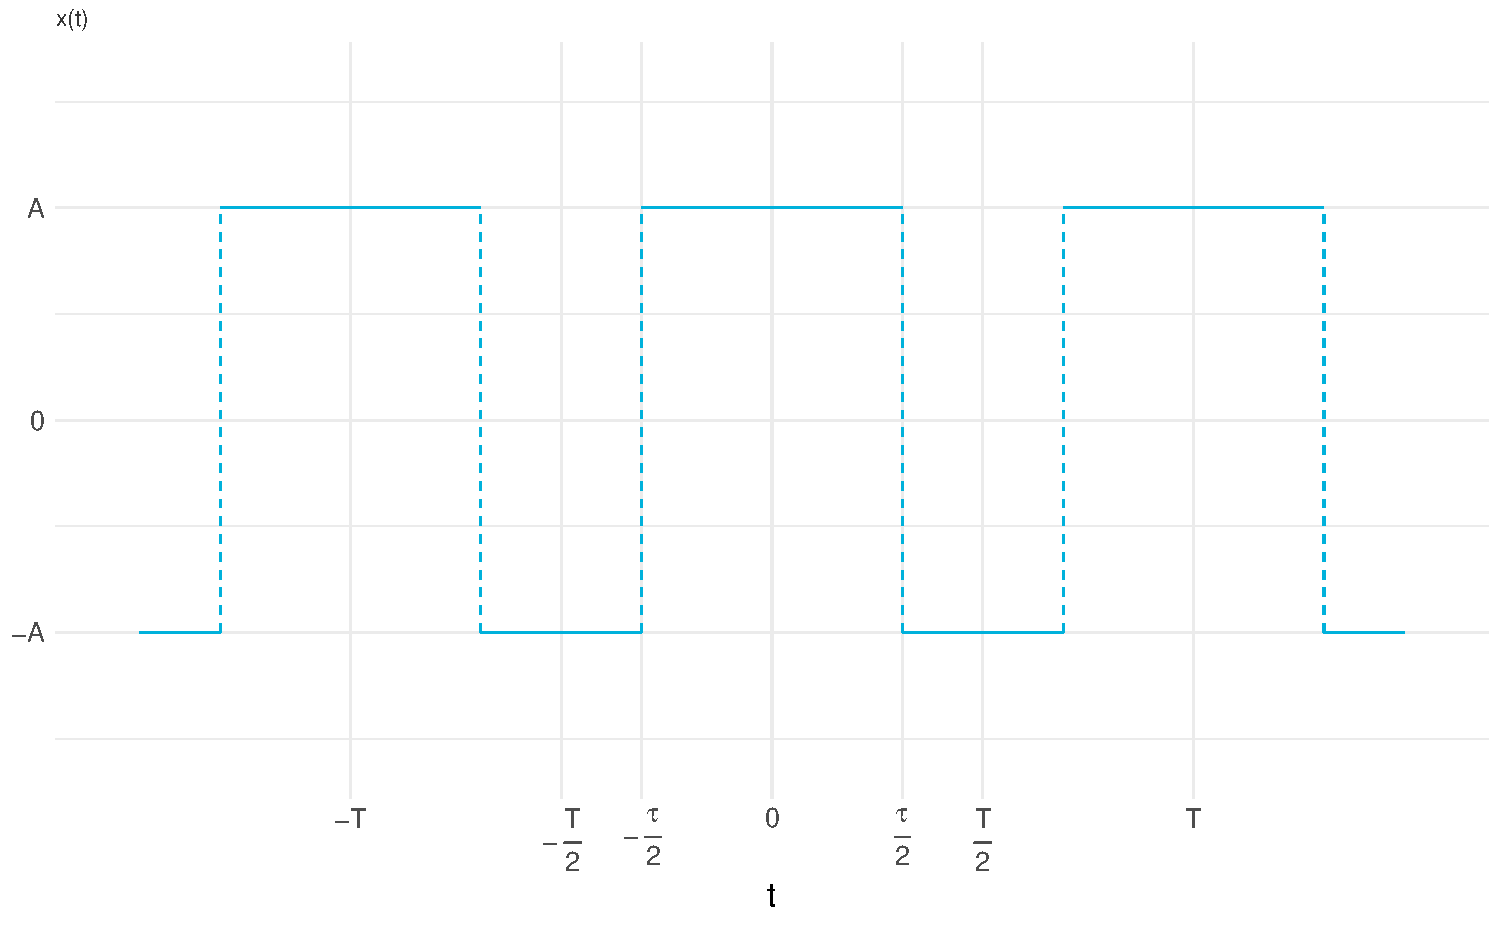
\includegraphics[width=\textwidth]{./1_1/1_1_function}


\begin{gather}
	\intertext{Hier gilt}
	x(t) = x(-t), \label{eq:1}\\
	\intertext{weshalb x(t) eine gerade Funktion ist. Damit ist}
	\nonumber
	b_n = \frac{2}{T} \int_T{ x(t) \cdot \sin{( n \omega_0 t)}  \dif t} = 0\\[\smallvert]
	\nonumber
	a_n = \frac{2}{T} \int_T{ x(t) \cdot \cos{( n \omega_0 t)}  \dif t} \\
	\nonumber
	= \frac{2}{T} 
	\left[
		\int_{-T/2}^{-\tau/2}{...}	 +
		\int_{-\tau/2}^{\tau/2}{...}+
		\int_{\tau/2}^{T/2}{...}
	\right]\\
	\intertext{mithilfe von Gl. \ref{eq:1}:}
	\nonumber
	a_n = \frac{2}{T}
	\left[
		2 \int_{0}^{\tau/2}{A \cdot \cos{( n \omega_0 t)}\dif t}+
		2 \int_{\tau/2}^{T/2}{-A \cdot \cos{( n \omega_0 t)}\dif t}
	\right]\\
	\nonumber
	= \frac{4 A}{T}
	\left[
		\int_{0}^{\tau/2}{\cos{( n \omega_0 t)}  \dif t} -
		\int_{\tau/2}^{T/2}{\cos{( n \omega_0 t)}  \dif t}
	\right]\\
	\nonumber
	= \frac{4 A}{T} \cdot \frac{1}{n \omega_0}
	\left[
		\sin{( n \omega_0 t )} \bigg\rvert_{0}^{\tau/2} -
		\sin{( n \omega_0 t )} \bigg\rvert_{\tau/2}^{T/2}
	\right]\\
	\intertext{mit $\omega_0 = \frac{2 \pi}{T}$:}
	\nonumber
	a_n = 
	\frac{4 A \cdot T}{T \cdot n 2 \pi}
	\left[ 
		\sin{(n \frac{2 \pi}{T} \frac{\tau}{2})} - 
		\left(
			\sin{(n \frac{2 \pi}{T} \frac{T}{2})} -
			\sin{(n \frac{2 \pi}{T} \frac{\tau}{2})}
		\right)
	\right]\\
	\nonumber
	= \frac{2 A}{n \pi}
	\left[ 
		\sin{(n \pi \frac{\tau}{T})} - 
		\underbrace{\sin{(n \pi)}}_{=0} +
		\sin{(n \pi \frac{\tau}{T})}
	\right]
\end{gather}

\eqbox{a_n = \frac{4 A}{n \pi} \cdot \sin{(n \pi \frac{\tau}{T})}}{0.382\textwidth}

\holine{0.618\textwidth}
%\noindent \textit{Berechnung des Gleichanteils}
\begin{gather*}
	a_0 = \frac{1}{T} \int_T{x(t) \dif t}\\
	\intertext{mithilfe von Gl. \ref{eq:1}:}
	a_0 = \frac{2}{T/2} \left[ \int_{0}^{\tau/2}{...} + \int_{\tau/2}^{T/2}{...} \right]\\
	= \frac{4 A}{T} \left[ t \bigg\rvert_{0}^{\tau/2} - t \bigg\rvert_{\tau/2}^{T/2}\right]\\
	= \frac{4 A}{T} \left[ \frac{\tau}{2} - \left( \frac{T}{2} - \frac{\tau}{2} \right)  \right]\\
	= \frac{4 A}{T} \left[ \tau - \frac{T}{2} \right]\\
	= 4 A \left[ \frac{\tau}{T} - \frac{1}{2} \right]
\end{gather*}

\eqbox{\frac{a_0}{2} = 2 A \left[ \frac{\tau}{T} - \frac{1}{2} \right]}{0.382\textwidth}


\holine{\textwidth}

\begin{gather*}
	\intertext{Für das Tastverhältnis $\frac{\tau}{T} = 0.5$  gilt:}
	\frac{a_0}{2} = 2 A \left[ \frac{1}{2} - \frac{1}{2}\right] = 0,\\
	a_n = \frac{4 A}{n \pi} \cdot \sin{(n \pi \frac{1}{2})} = \frac{4 A}{n \pi} \cdot \sin{(n \frac{\pi}{2})}\\
	a_n = \frac{4 A}{n \pi} \cdot (-1)^{n+1}
\end{gather*}

\begin{figure}[H]
  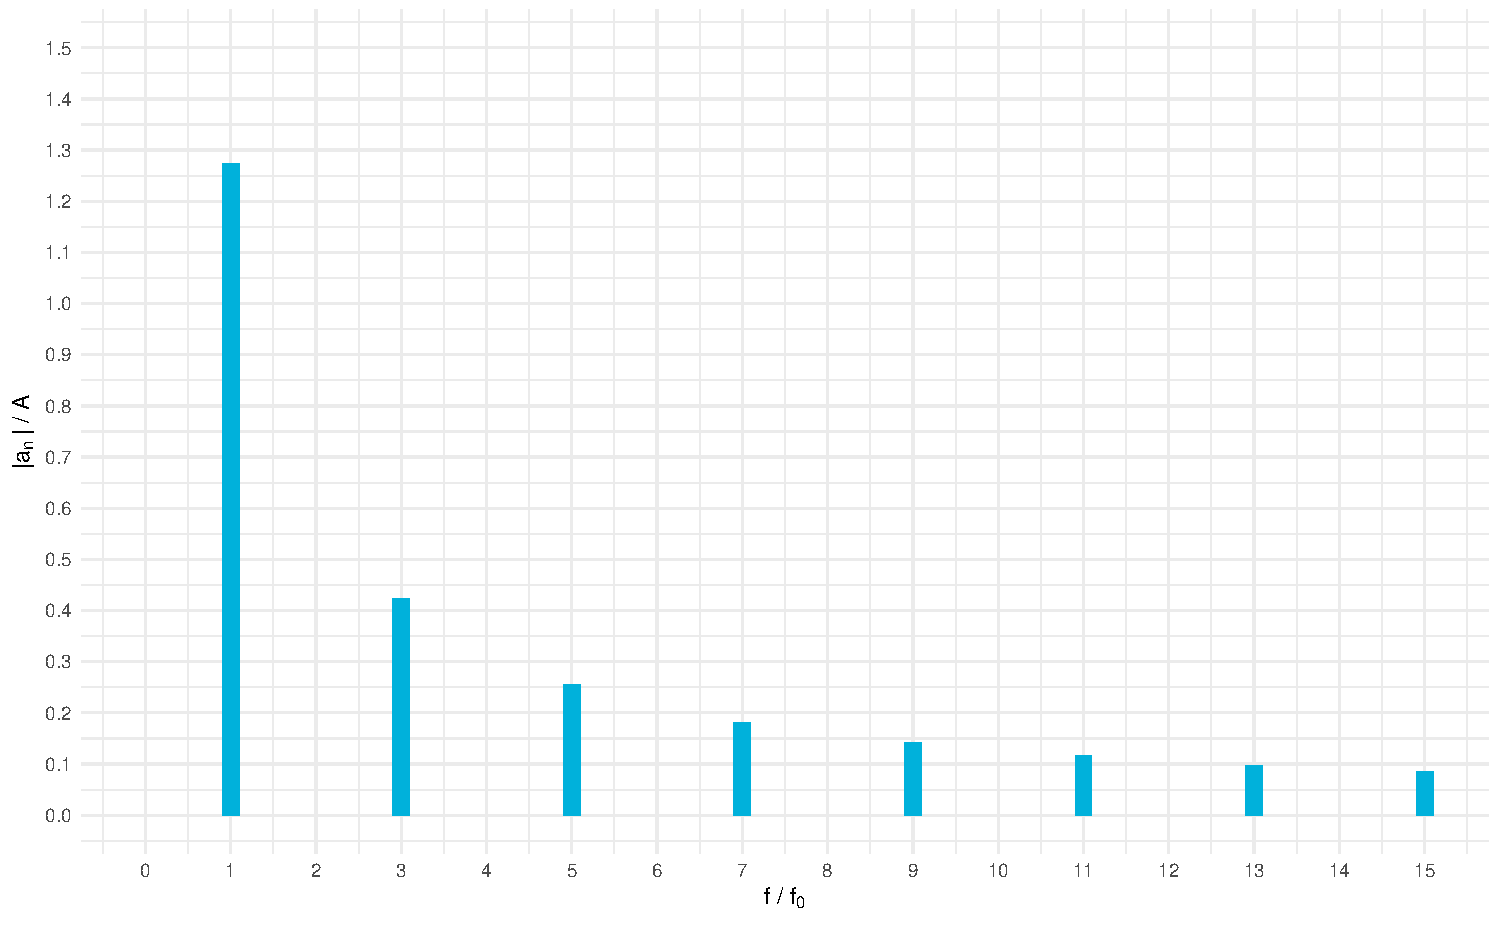
\includegraphics[width=\textwidth]{1_1/1_1_AS}
	\caption{Betragsspektrum von x(t) für $\frac{\tau}{T} = 0.5$}
\end{figure}

%%%%%%%%%%%%%%%%%%%%%%%
\subsection{}

\begin{figure}[H]
  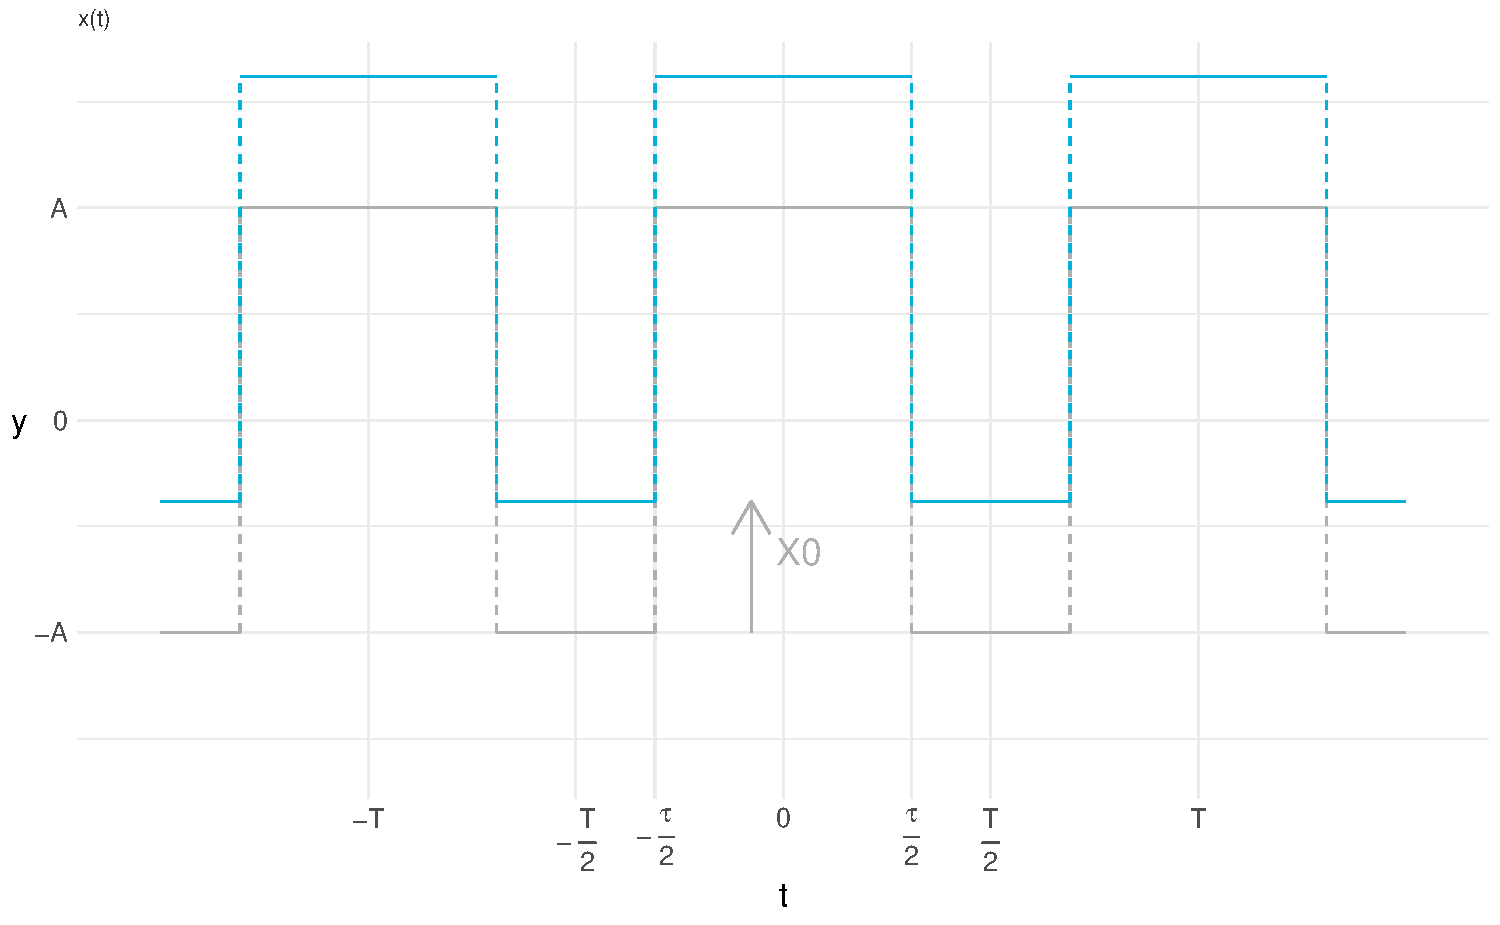
\includegraphics[width=\textwidth]{1_2/1_2_function}
	\caption{x(t) mit dem Gleichanteil X0 im Zeitbereich}
\end{figure}

\begin{gather*}
  \intertext{Auswirkungen im Frequenzbereich:}
  a_n = \frac{2}{T} \int_{T}{(x(t) + X0) \cdot \cos{(n \omega_0 t)}\dif t}\\
      = \frac{2}{T} \left[  \int_{T}{x(t) \cos{(n\omega_0 t)} \dif t}+
        \underbrace{\int_T{X0 \cdot
          \cos{(n \omega_0 t)} \dif t}}_{=0} \right]\\
  a_n = \frac{2}{T} \int_{T}{x(t) \cdot \cos{(n \omega_0 t)}\dif t}\\
  \intertext{$\rightarrow$ Im Frequenzbereich finden keine Änderungen statt.}
  \intertext{$\rightarrow$ Nur der Gleichanteil ändert sich}
\end{gather*}

\subsection{}

\begin{gather*}
	\intertext{Für das Tastverhältnis $\frac{\tau}{T} = 0.25$  gilt:}
	\frac{a_0}{2} = 2 A \left[ \frac{1}{4} - \frac{1}{2}\right] = - A ,\\
	a_n = \frac{4 A}{n \pi} \cdot \sin{(n \pi \frac{1}{4})}\\
	a_n = \frac{4 A}{n \pi} \cdot \sin{(n \frac{\pi}{4})}
\end{gather*}

\begin{figure}[H]
  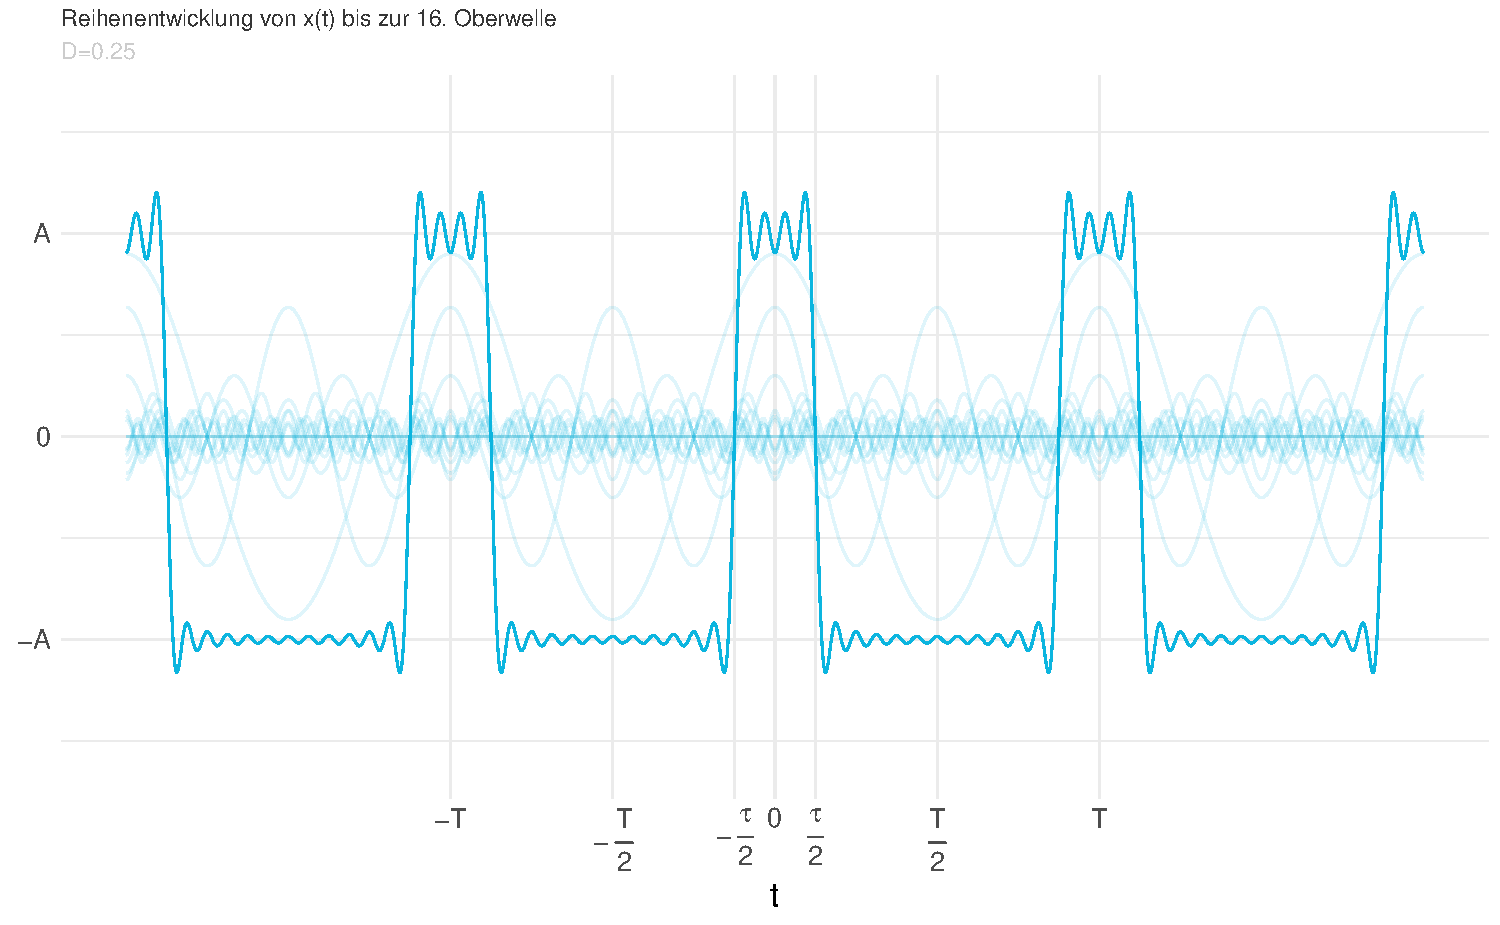
\includegraphics[width=\textwidth]{1_3/1_3_Reihe}
	\caption{x(t) als Summe der Einzelschwingungen}
\end{figure}


\subsection{}
\begin{figure}[H]
  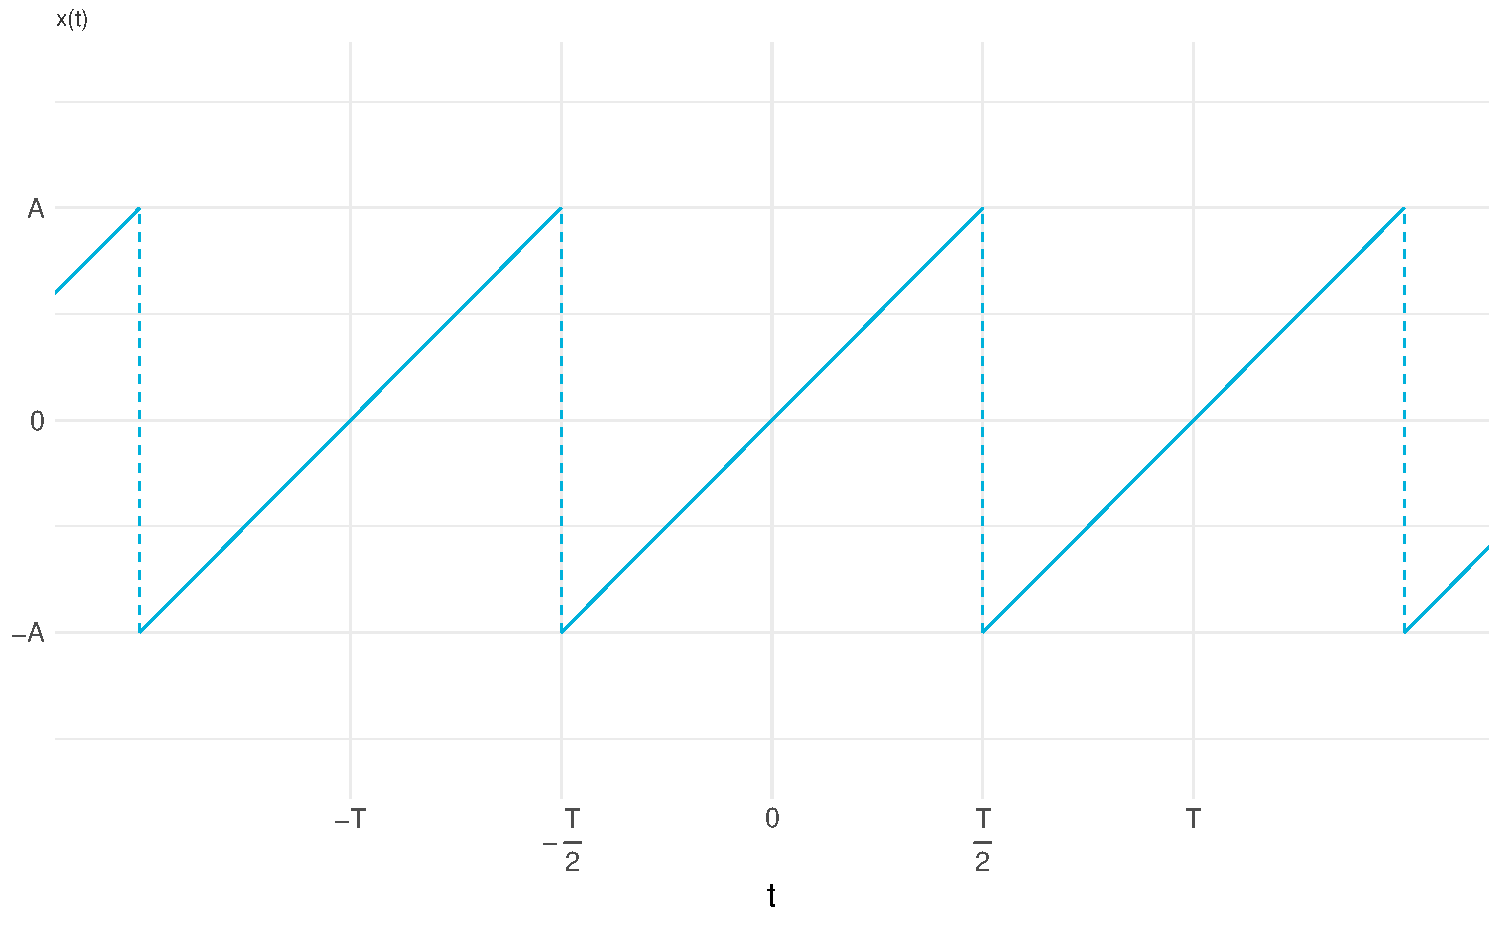
\includegraphics[width=\textwidth]{1_4/1_4_function}
\end{figure}



\begin{gather}
	\intertext{Es gilt:}
	x(-t) = -x(t),\\
	\intertext{weshalb $x(t)$ eine ungerade Funktion ist. Damit ist}
	\nonumber
	a_n = \frac{2}{T} \int_T{x(t) \cdot \cos{(n \omega_0 t)} \dif t} = 0\\
  \intertext{und}
	 \nonumber
  a_0 = \frac{1}{T} \int^{T/2}_{-T/2}{x(t) \dif t} = 0\\[\smallvert]
\nonumber
	b_n = \frac{2}{T} \int_T{x(t) \cdot \sin{(n \omega_0 t)} \dif t}\\
 	\nonumber
	= \frac{2}{T}
		\int_{-T/2}^{T/2}{ \frac{A}{T/2} \cdot t \cdot \sin{(n \omega_0 t)} \dif t}\\
	\nonumber
	= \frac{4 A }{T^2}
		\int_{-T/2}^{T/2}{ t \cdot \sin{(n \omega_0 t)} \dif t}\\
	\intertext{Partielle Integration:}
	\nonumber
	u = t, u' = 1\\
	\nonumber
	v' = \sin{(n\omega_0 t)}, v = - \frac{1}{n \omega_0} \cdot \cos{(n\omega_0 t)}\\
	\nonumber
	b_n = \frac{4 A}{T^2} \left[ - \frac{1}{n \omega_0} \cdot \left[ t \cos{n\omega_0 t} \right]\bigg\rvert_{-T/2}^{T/2} + \frac{1}{n \omega_0} \int_{-T/2}^{T/2}{ \cos(n \omega_0 t) \dif t  } \right]\\
	\intertext{mit $\omega_0 = \frac{2 \pi}{T}$}
	\nonumber
	= \frac{4 A}{T^2} \left[ 
	- \frac{1}{n \omega_0} \cdot \left[ \frac{T}{2} \cos{(n \frac{2 \pi T}{T^2})}-(-\frac{T}{2} \cos{(- n \frac{2 \pi T}{T^2})}) \right]+ \frac{1}{n^2 \omega_0^2}\left[ \sin{(n \omega_0 t)} \right]\bigg\rvert_{-T/2}^{T/2}
	\right]\\
	\nonumber
	= \frac{4 A}{T^2} \left[
	- \frac{1}{n \omega_0} \cdot \left[ \frac{T}{2} \cos{(n \pi)} + \frac{T}{2} \cos{(n \pi)} \right]+ \frac{1}{n^2 \omega_0^2}\underbrace{\left[ \sin{(n \frac{2 \pi}{T} t)} \right]\bigg\rvert_{-T/2}^{T/2}}_{=0}
	\right]\\
	\nonumber
	= - \frac{4 A}{T^2 n \omega_0} \cdot \frac{2 T }{2} \left[
		\cos{(n \pi)}
	\right]\\
	\nonumber
	= -\frac{2 A}{n \pi} (-1)^n
\end{gather}

\eqbox{b_n = \frac{2A}{n \pi} \cdot (-1)^{n+1}}{0.382\textwidth}

\begin{figure}[H]
  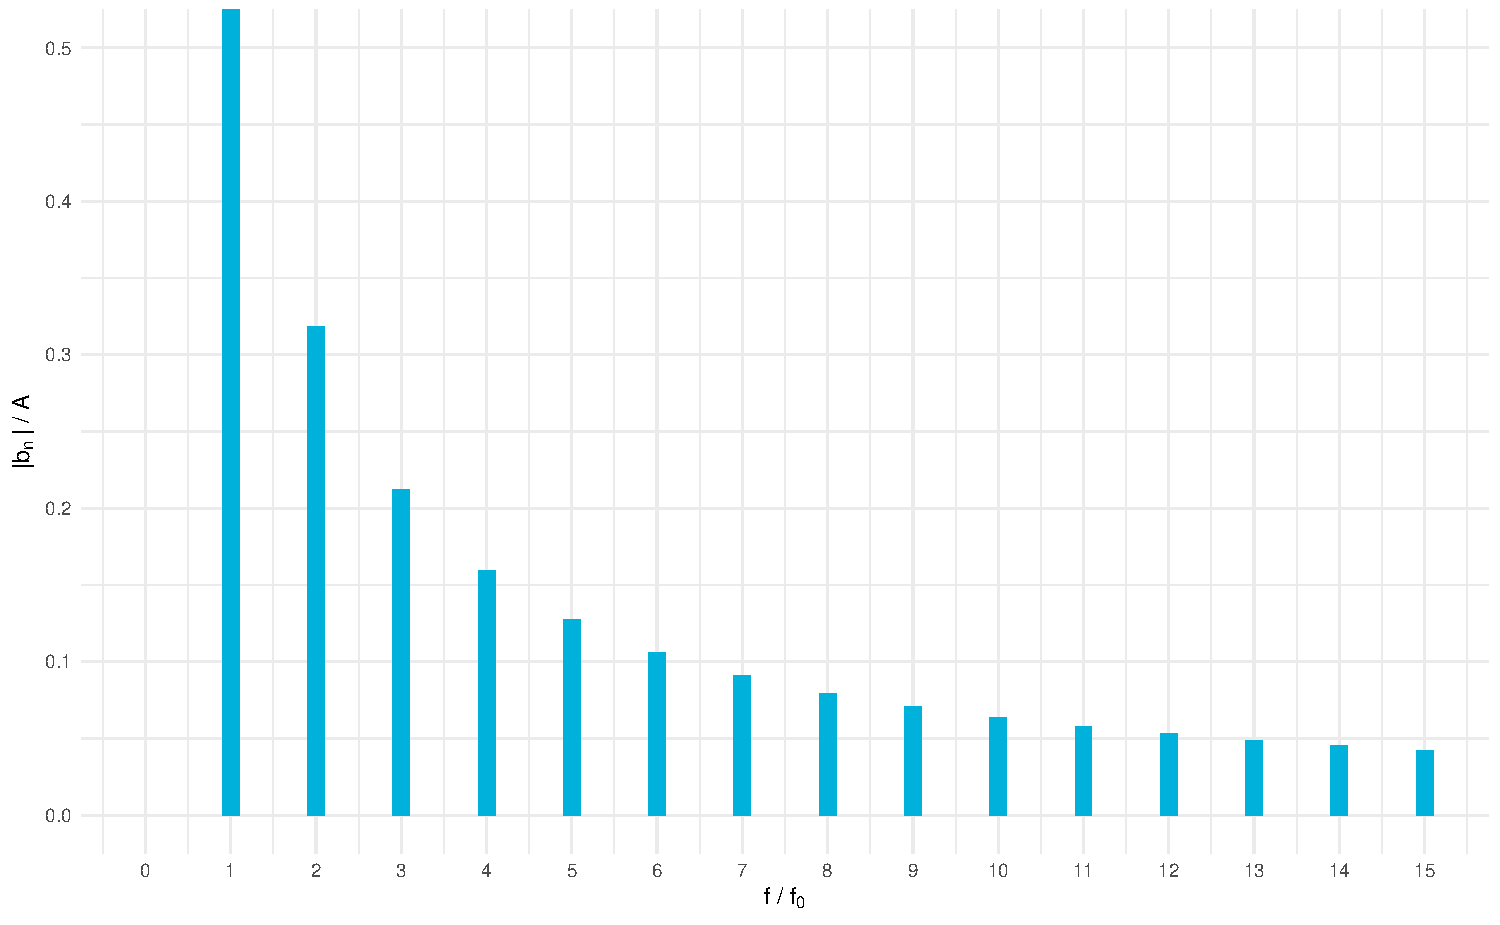
\includegraphics[width=\textwidth]{1_4/1_4_AS}
  \caption{Betragsamplitudenspektrum von x(t)}
\end{figure}

\begin{figure}[H]
  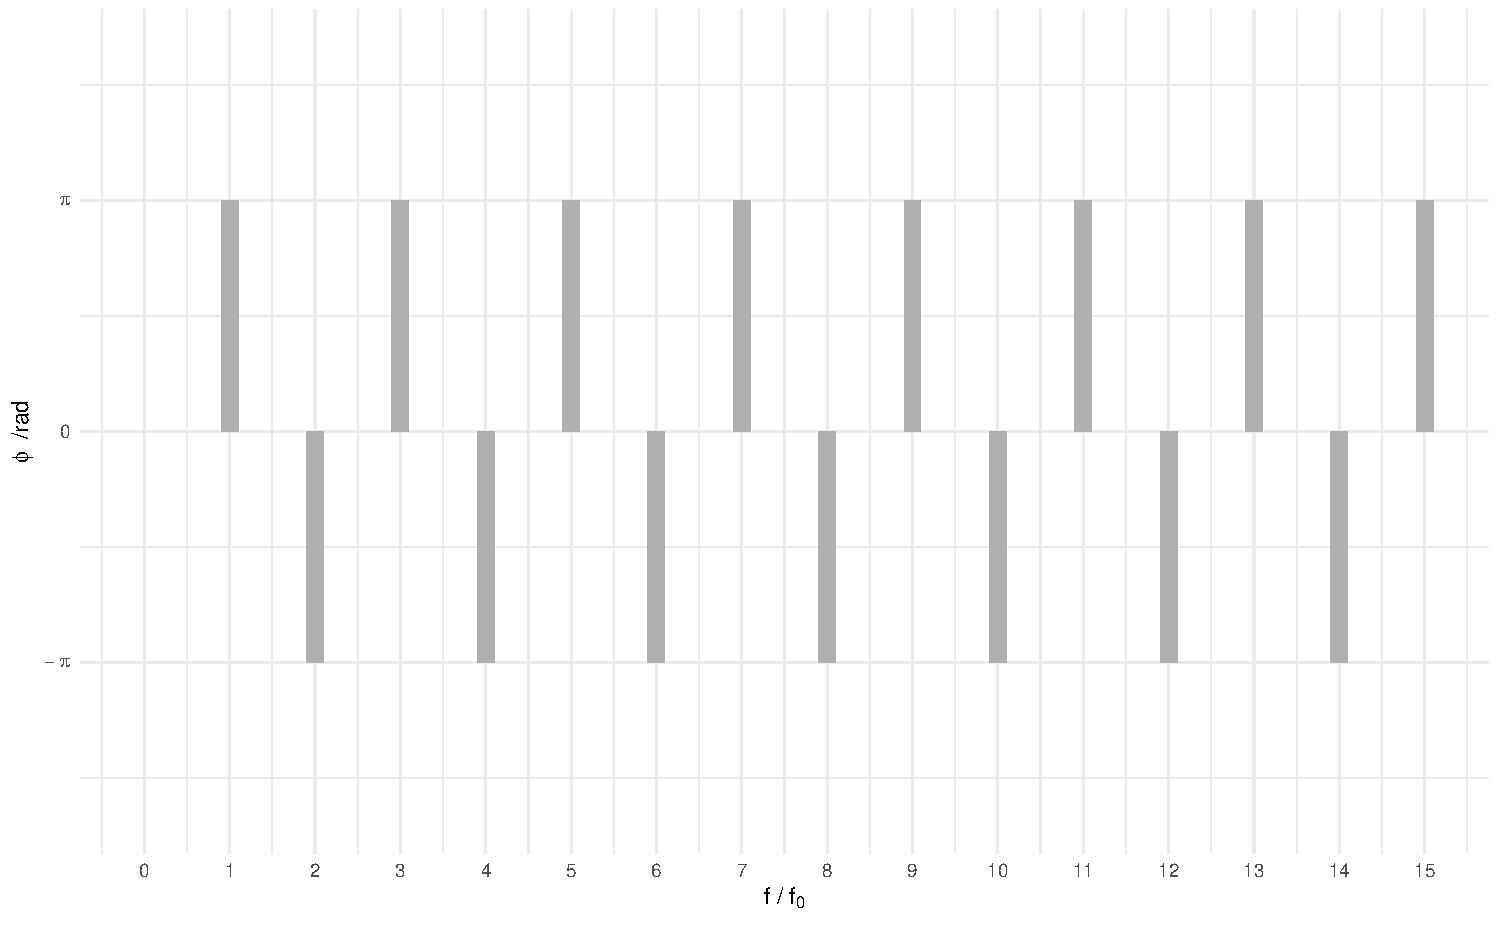
\includegraphics[width=\textwidth]{1_4/1_4_Phase}
  \caption{Phasenspektrum von x(t)}
\end{figure}

\section{Versuchsaufgaben}

% 2.1
\subsection{}

Aufgrund des Verhaltens des Signalgenerators (Betriebssystem, AgilentVEE-Software, PC-Soundkarte) konnte keine genaue Amplitude des Sinussignals von $\pm 2 \,\ \si{\volt}$ eingestellt und dadurch auch nicht am Oszilloskop nachvollzogen werden. Daher lässt sich auch kein Vergleich der generierten und gemessenen Amplituden erstellen.

\noindent Aus Abbildung 6 kann man bei einer Einteilung von $200 \frac{\si{\micro\second}}{\textrm{division}}$ eine Periodendauer von etwa $500 \,\ \si{\micro\second}$ erkennen. Die Frequenz
$$ f = \frac{1}{500 \si{\micro\second}} = 2 \,\ \si{\kilo\hertz}$$
ist damit nachvollziehbar.

\begin{figure}[H]
  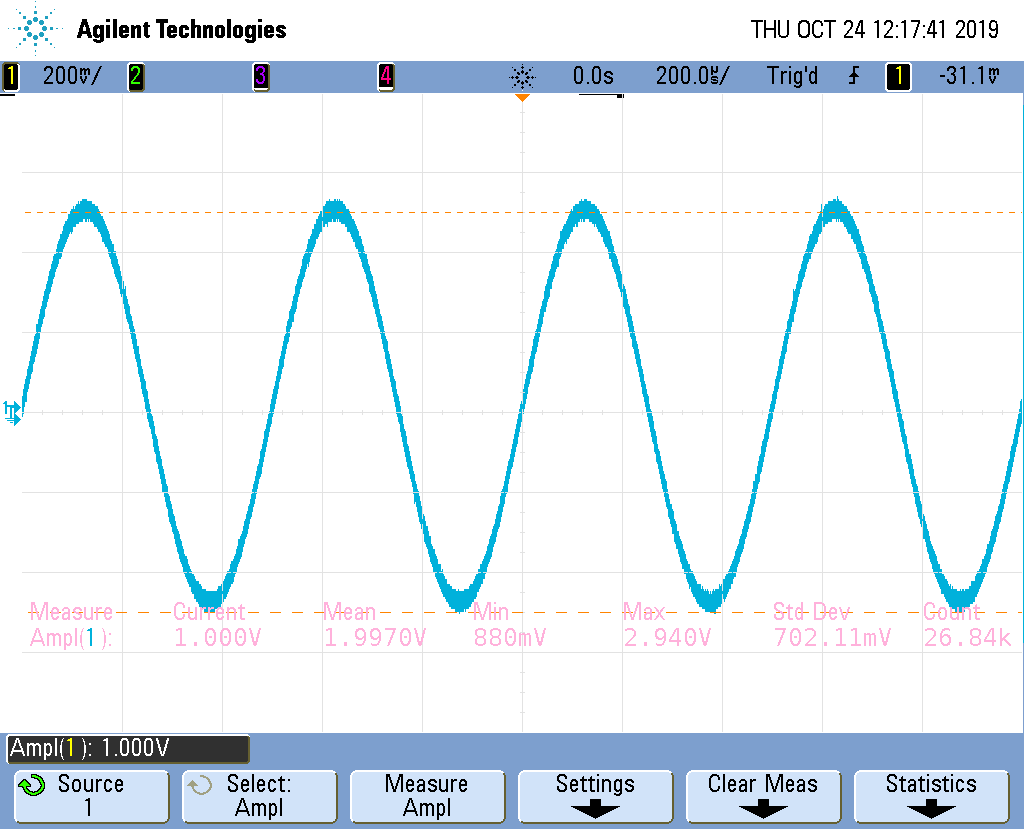
\includegraphics[width=\textwidth]{2_1/scope_0_blue}
  \caption{Screenshot des Sinussignals auf dem Oszilloskop}
\end{figure}

% 2.2
\subsection{}

\begin{gather*}
	\intertext{Analytische Bestimmung des Amplitudenspektrums, Aus 1.1 ergibt sich:}
  D = \frac{\tau}{T} = \frac{1}{2}\\
  \frac{a_0}{2} = 0
\end{gather*}

\begin{gather*}
	a_n = \frac{4 \cdot 2 \si{\volt}}{n \pi}\cdot (-1)^{n+1}\\
\end{gather*}

\begin{table}[H]
\begin{center}
\begin{tabular}{@{}cccc@{}}
\toprule
$f/\si{\kilo\hertz}$ & $a_n / \si{\volt}$ & $b_n / \si{\volt}$ \\ \midrule
1                      &  2.457     & 0     \\
2                      &  0     & 0     \\
3                      &  -0.849     & 0     \\
4                      &  0     & 0     \\
5                      &  0.509     & 0     \\
6                      &  0     & 0     \\
7                      &  -0.364     & 0     \\
8                      &  0    & 0     \\
9                      &  0.283     & 0     \\
10                     &  0    & 0     \\ \bottomrule
\end{tabular}
\end{center}
\caption{Fourierkoeffizienten $D = 0.5$}
\end{table}

\noindent Aus Abbildung 7 kann man bei einer Einteilung von $200 \frac{\si{\micro\second}}{\textrm{division}}$ eine Periodendauer von etwa $1000 \,\ \si{\micro\second}$ erkennen. Die Periodendauer ist also wie eingestellt. Wie in 2.1 bereits erwähnt lassen sich keine Rückschlüsse auf die Amplitude treffen. Die Impulsdauer ist mit $ 500 \,\ \si{\micro\second}$ ebenfalls wie eingestellt und ergibt zusammen mit der Periodendauer ein Tastverhältnis von $D = 0.5$.

\noindent Des Weiteren ist das Überschwingen (\textit{Gibbs'sches Phänomen}) deutlich aus dem Oszilloskopbild ersichtlich.


\begin{figure}[H]
  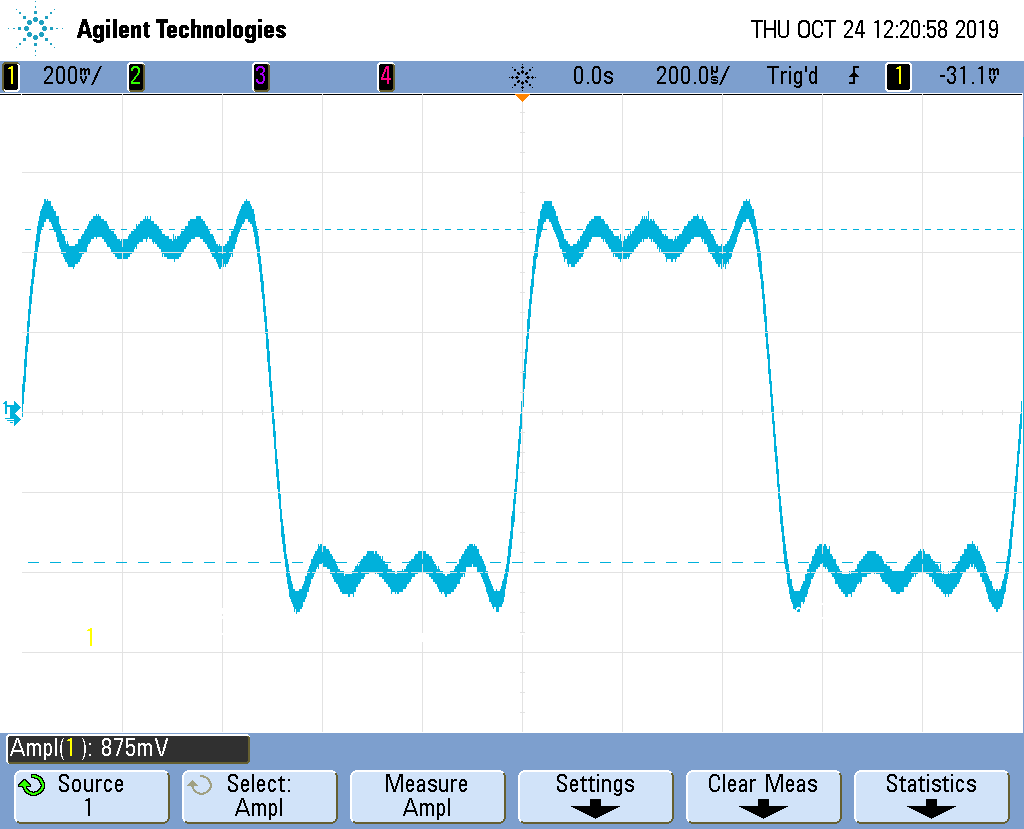
\includegraphics[width=\textwidth]{2_2/scope_1_blue}
  \caption{Screenshot des Rechtecksignals ($D = 0.5$) auf dem Oszilloskop}
\end{figure}


\noindent Die theoretische Fouriersynthese eines Signals besteht aus unendlich vielen Summengliedern. Da dies praktisch nicht möglich ist und man nur eine begrenzte Anzahl an Oberwellen synthetisieren kann, ist die Qualität des resultieren Signals von dieser begrenzten Anzahl abhängig. Im Versuch wurden maximal 9 Oberwellen verwendet, wodurch die Approximation des Rechtecksignals fehlerbehaftet ist. 

\noindent Die Soundkarte des PCs filtert die im Programm eingestellten Gleichanteile, sodass sie in der Messung nicht erkennbar waren.

\begin{figure}[H]
  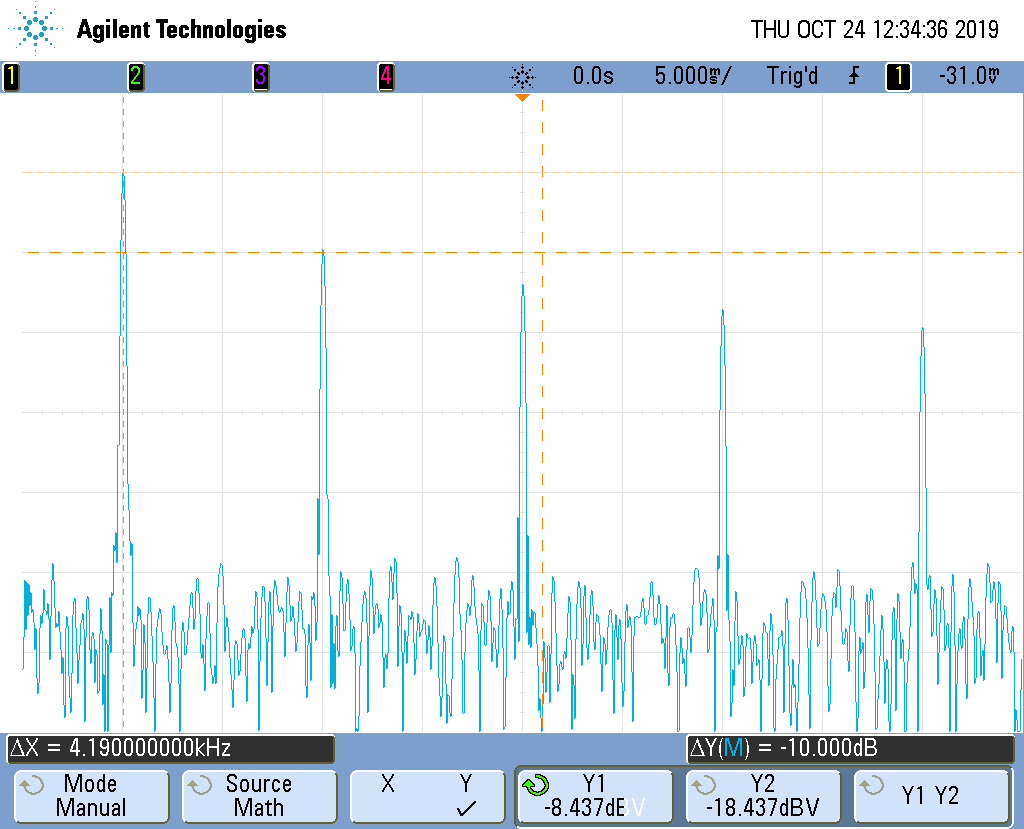
\includegraphics[width=\textwidth]{2_2/scope_2_white}
  \caption{Screenshot des Amplitudenspektrums auf dem Oszilloskop}
\end{figure}

\begin{table}[H]
  \begin{center}
\begin{tabular}{@{}cccc@{}}
\toprule
$n_1-n_2$ & $\Delta a_{\textrm{theoretisch}} / \si{\deci\bel}$ & $\Delta a_{\textrm{gemessen}} / \si{\deci\bel}$ & $\Delta a_{\textrm{theoretisch}} - \Delta a_{\textrm{gemessen}}/ \si{\deci\bel}$  \\ \midrule
1-3       &  -9.229                       & -10                         &   0.771         \\
3-5       &  -4.444                       & -3.75                       &  0.694          \\
5-7       &  -2.912                      & -2.81                      &     0.102       \\
7-9       &  -2.004                       & -2.5                        &  0.496          \\ \bottomrule
\end{tabular}
\caption{Messwerte der Aufgabe 6.2}
\end{center}
\end{table}

\noindent Die Bestimmung der theoretischen Werte $\Delta a_{\textrm{theoretisch}}$ in dB erfolgte durch
$$\Delta a_{\textrm{theoretisch}} = 20 \cdot \log{\frac{a_n}{a_{n-1}}}$$

\noindent Die Abweichungen der gemessenen und theoretischen Amplitudendifferenzen sind nicht unerheblich. Die Ursache liegt u.a. bei dem willkürlichen Anlegen des Cursors auf dem Oszilloskop sowie anderen zufälligen Messabweichungen.


\noindent (Anmerkung zur Messwertaufnahme bzgl. Tabelle 2: Durch Messung der Differenzen gegen eine konstanten Bezugspunkt (z.B. Cursor an $a_1$), hätte sich der Fehler minimieren lassen können.)

\begin{figure}[H]
  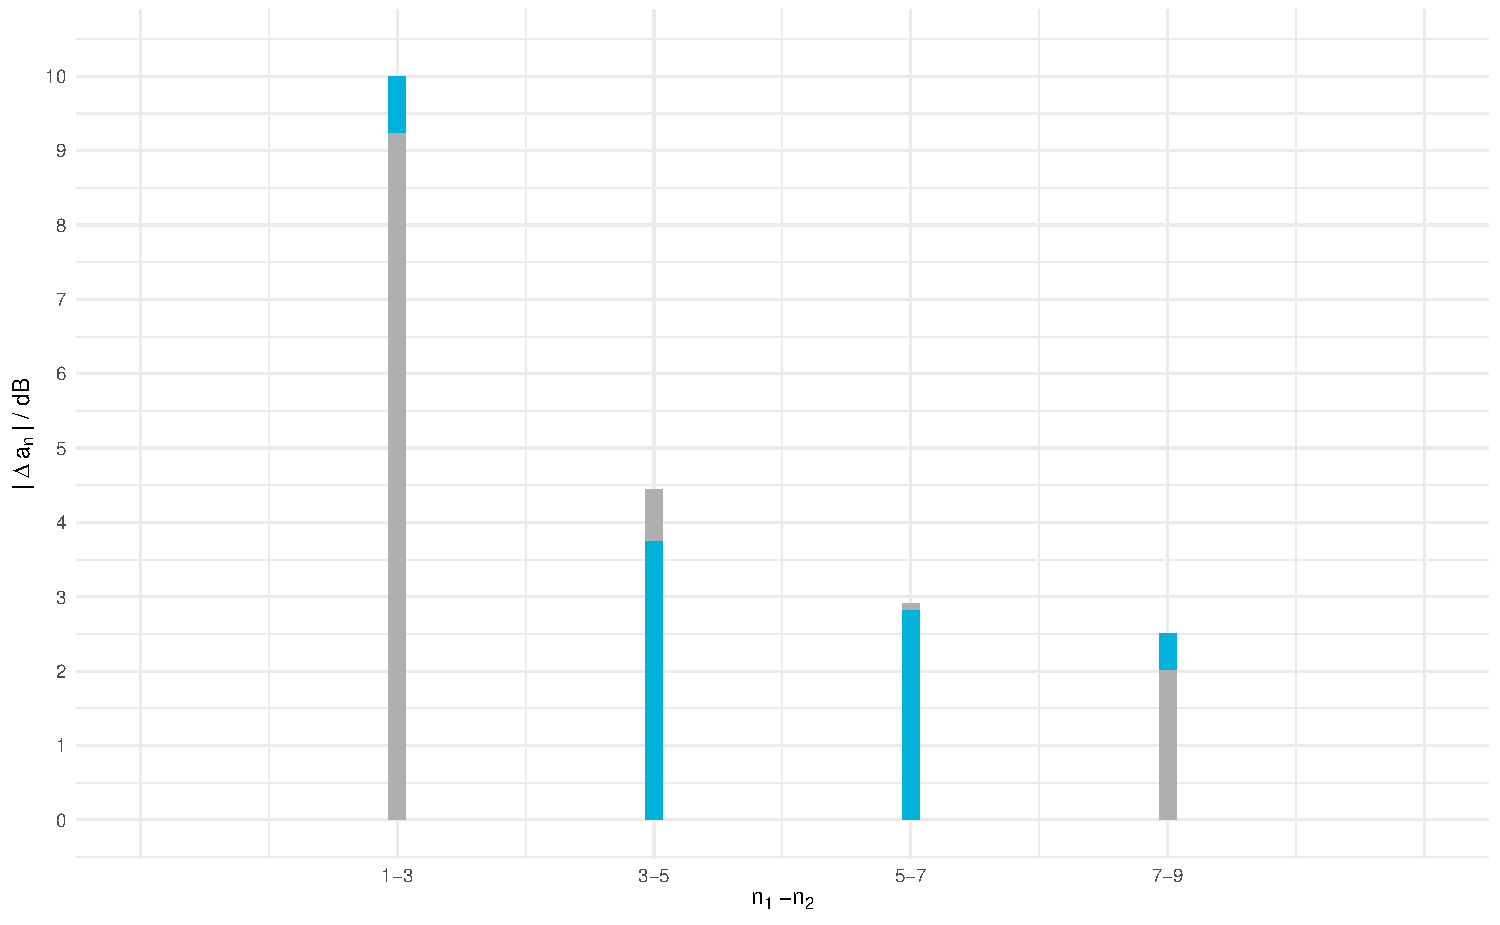
\includegraphics[width=\textwidth]{2_2/2_2_Amplivergleich}
  \caption{Vergleich der theoretischen (grau) und gemessenen (blau) Werte }
\end{figure}


% 2.3
\subsection{}

\begin{gather*}
  \intertext{Aus 1.3 folgt}
  \frac{a_0}{2} = -A = -2 \,\ \si{\volt}\\
  a_n = \frac{4 \cdot 2 \si{\volt}}{ n \pi } \cdot \sin{(n \pi \frac{1}{4})}
\end{gather*}

\begin{table}[H]
\begin{center}
\begin{tabular}{@{}cccc@{}}
\toprule
$f/\si{\kilo\hertz}$ & $a_n / \si{\volt}$ & $b_n / \si{\volt}$ \\ \midrule
1                      &  1.801     & 0     \\
2                      &  1.273     & 0     \\
3                      &  0.600     & 0     \\
4                      &  0     & 0     \\
5                      &  -0.360     & 0     \\
6                      &  -0.424     & 0     \\
7                      &  -0.257     & 0     \\
8                      &  0    & 0     \\
9                      &  0.200     & 0     \\
10                     &  0.255    & 0     \\ \bottomrule
\end{tabular}
\end{center}
\caption{Fourierkoeffizienten $D = 0.25$}
\end{table}

\begin{table}[H]
	\begin{center}
		\begin{tabular}{@{}cccc@{}}
			\toprule
			$n_1-n_2$ & $\Delta a_{\textrm{theoretisch}} / \si{\deci\bel}$ & $\Delta a_{\textrm{gemessen}} / \si{\deci\bel}$ & $\Delta a_{\textrm{theoretisch}} - \Delta a_{\textrm{gemessen}}/ \si{\deci\bel}$  \\ \midrule
			1-2       &  -3.013                       & -2.969                         &   0.044         \\
			2-3       &  -6.534                       & -6.718                         &   -0.184         \\
			3-5       &  -4.437                       & -4.375                         &   0.062         \\
			5-6       &  1.421                       & 1.094                       & 0.327         \\
			6-7       &  -4.349                      & -3.75                      &     -0.689       \\
			7-9       &  -2.178                       & -2.813                        &  0.635          \\ \bottomrule
		\end{tabular}
		\caption{Messwerte der Aufgabe 6.3}
	\end{center}
\end{table}

\noindent Berechnungen und Fehler ergeben sich wie in 2.2.

\begin{figure}[H]
  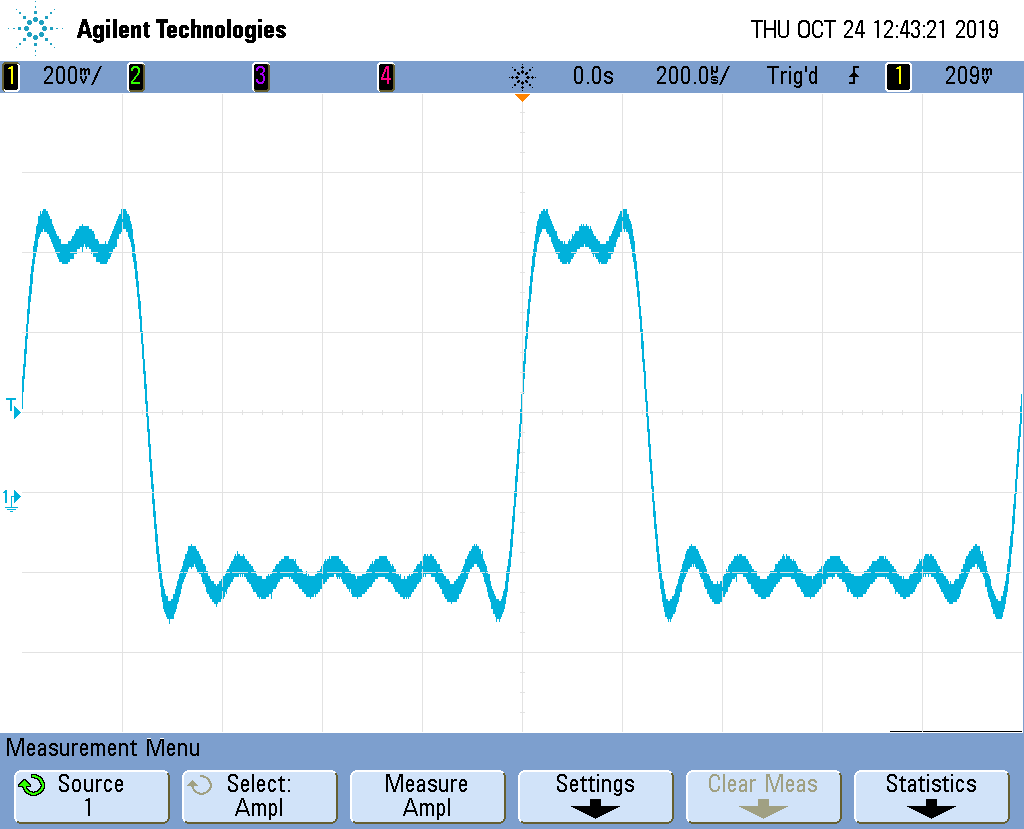
\includegraphics[width=\textwidth]{2_3/scope_3_blue}
  \caption{Screenshot des Rechtecksignals ($D = 0.25$) auf dem Oszilloskop}
\end{figure}

\begin{figure}[H]
  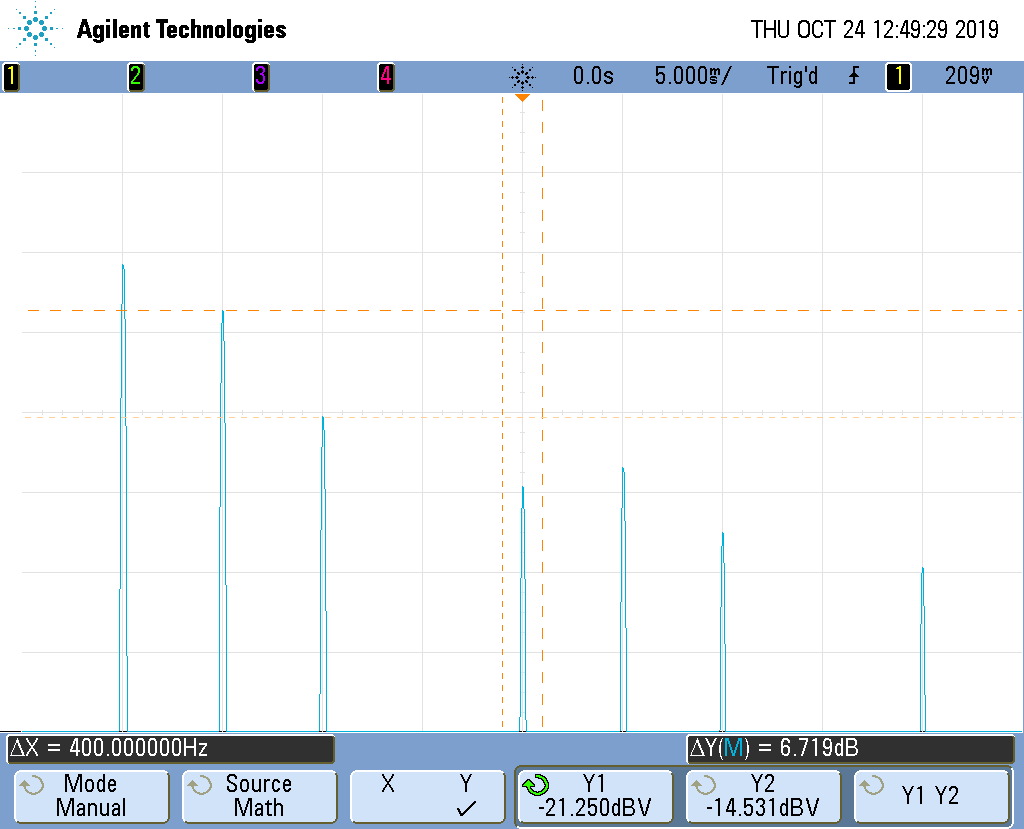
\includegraphics[width=\textwidth]{2_3/scope_4_white}
  \caption{Screenshot des Amplitudenspektrums auf dem Oszilloskop}
\end{figure}

\noindent Aus Abbildung 11 lässt sich erkennen, dass sich bei verringertem Tastverhältnis die Dichte der spektralen Amplituden erhöht, wie es auch erwartet wurde.

\begin{figure}[H]
  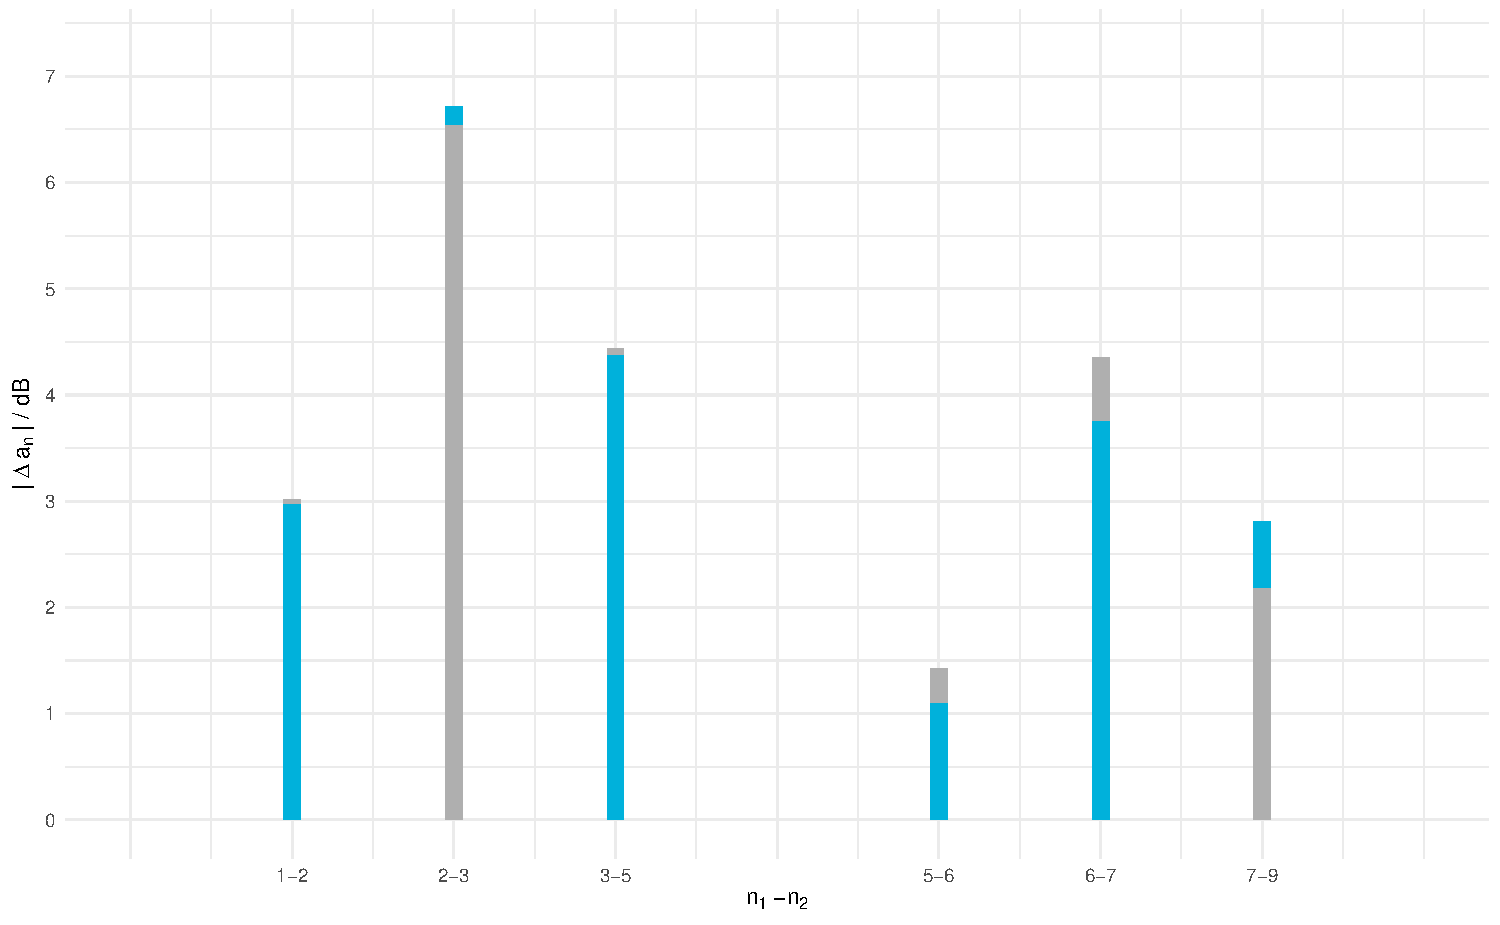
\includegraphics[width=\textwidth]{2_3/2_3_Amplivergleich}
  \caption{Vergleich der theoretischen (grau) und gemessenen (blau) Werte }
\end{figure}


% 2.4
\subsection{}

\begin{table}[H]
\begin{center}
\begin{tabular}{@{}cccc@{}}
\toprule
$f/\si{\kilo\hertz}$ & $a_n / \si{\volt}$ & $b_n / \si{\volt}$ \\ \midrule
1                      &  0       & 1.273   \\
2                      &  0     & -0.637    \\
3                      &  0     & 0.424     \\
4                      &  0     & -0.318    \\
5                      &  0     & 0.255     \\
6                      &  0     & -0.212    \\
7                      &  0     & 0.182     \\
8                      &  0    & -0.159     \\
9                      &  0     & 0.141     \\
10                     &  0    & -0.127     \\ \bottomrule
\end{tabular}
\end{center}
\caption{Fourierkoeffizienten der Sägezahnfunktion}
\end{table}

\begin{table}[H]
	\begin{center}
		\begin{tabular}{@{}cccc@{}}
			\toprule
			$n_1-n_2$ & $\Delta b_{\textrm{theoretisch}} / \si{\deci\bel}$ & $\Delta b_{\textrm{gemessen}} / \si{\deci\bel}$ & $\Delta b_{\textrm{theoretisch}} - \Delta b_{\textrm{gemessen}}/ \si{\deci\bel}$  \\ \midrule
			1-2       &  -6.010                       & -6.531                         &   -0.521         \\
			2-3       &  -3.536                       & -3.094                        &   0.442         \\
			3-4       &  -2.499                       & -2.75                         &   -0.251         \\
			4-5       &  -1.918                       & -2.062                         &   -0.144         \\
			5-6       &  -1.604                       & -1.75                       & 0.146         \\
			6-7       &  -1.325                      & -1.531                      &     0.206       \\
			7-8       &  -1.173                       & -1.094                         &   -0.079         \\
			8-9       &  -1.044                       & -0.875                        &  -0.169          \\ \bottomrule
		\end{tabular}
		\caption{Messwerte der Aufgabe 6.4}
	\end{center}
\end{table}

\begin{figure}[H]
  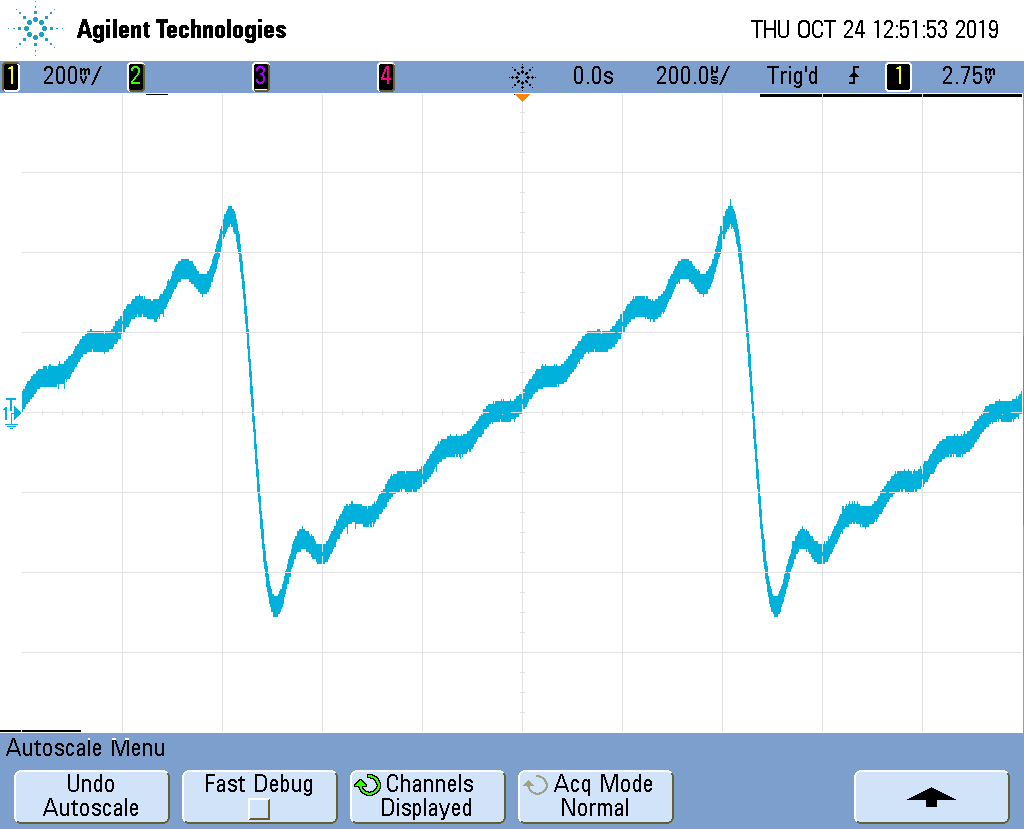
\includegraphics[width=\textwidth]{2_4/scope_5_blue}
  \caption{Screenshot des Sägezahnsignals auf dem Oszilloskop}
\end{figure}

\begin{figure}[H]
  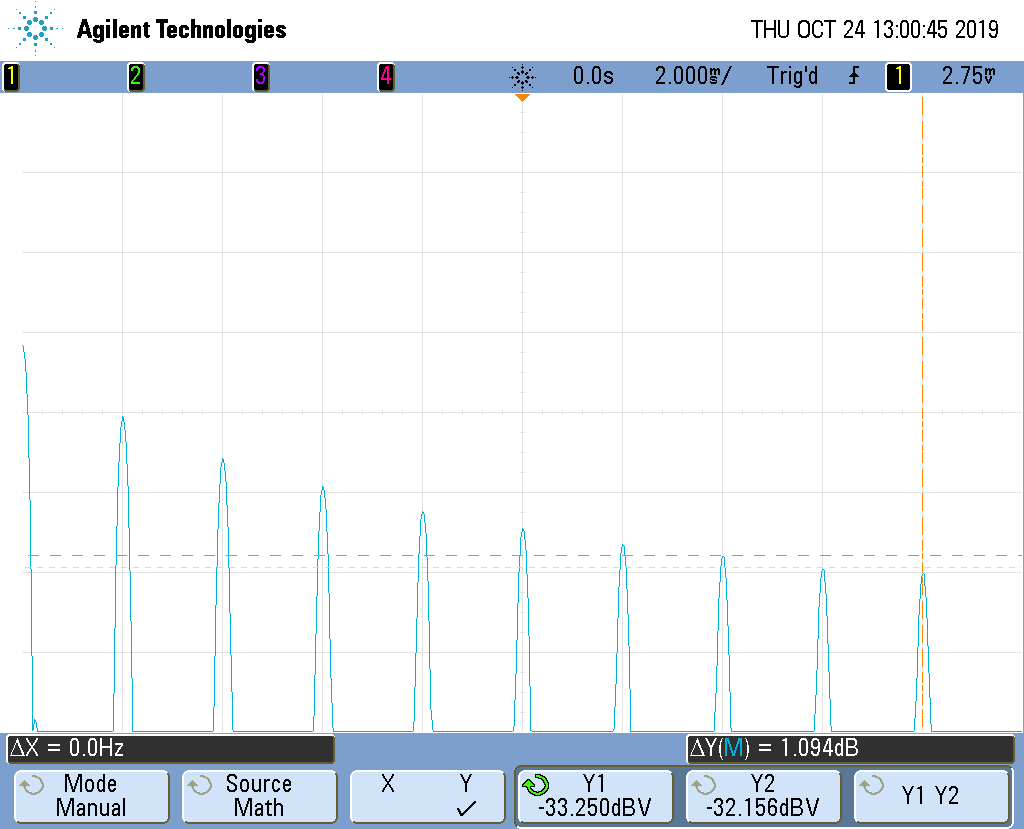
\includegraphics[width=\textwidth]{2_4/scope_6_white}
  \caption{Screenshot des Amplitudenspektrums auf dem Oszilloskop}
\end{figure}

\noindent Wie erwartet fallen die spektralen Amplituden hyperbolisch ($\propto \frac{1}{n}$) ab. Die Abweichungen befinden sich wieder in der gleichen Größenordnung wie bei den Messungen zuvor. 

\begin{figure}[H]
  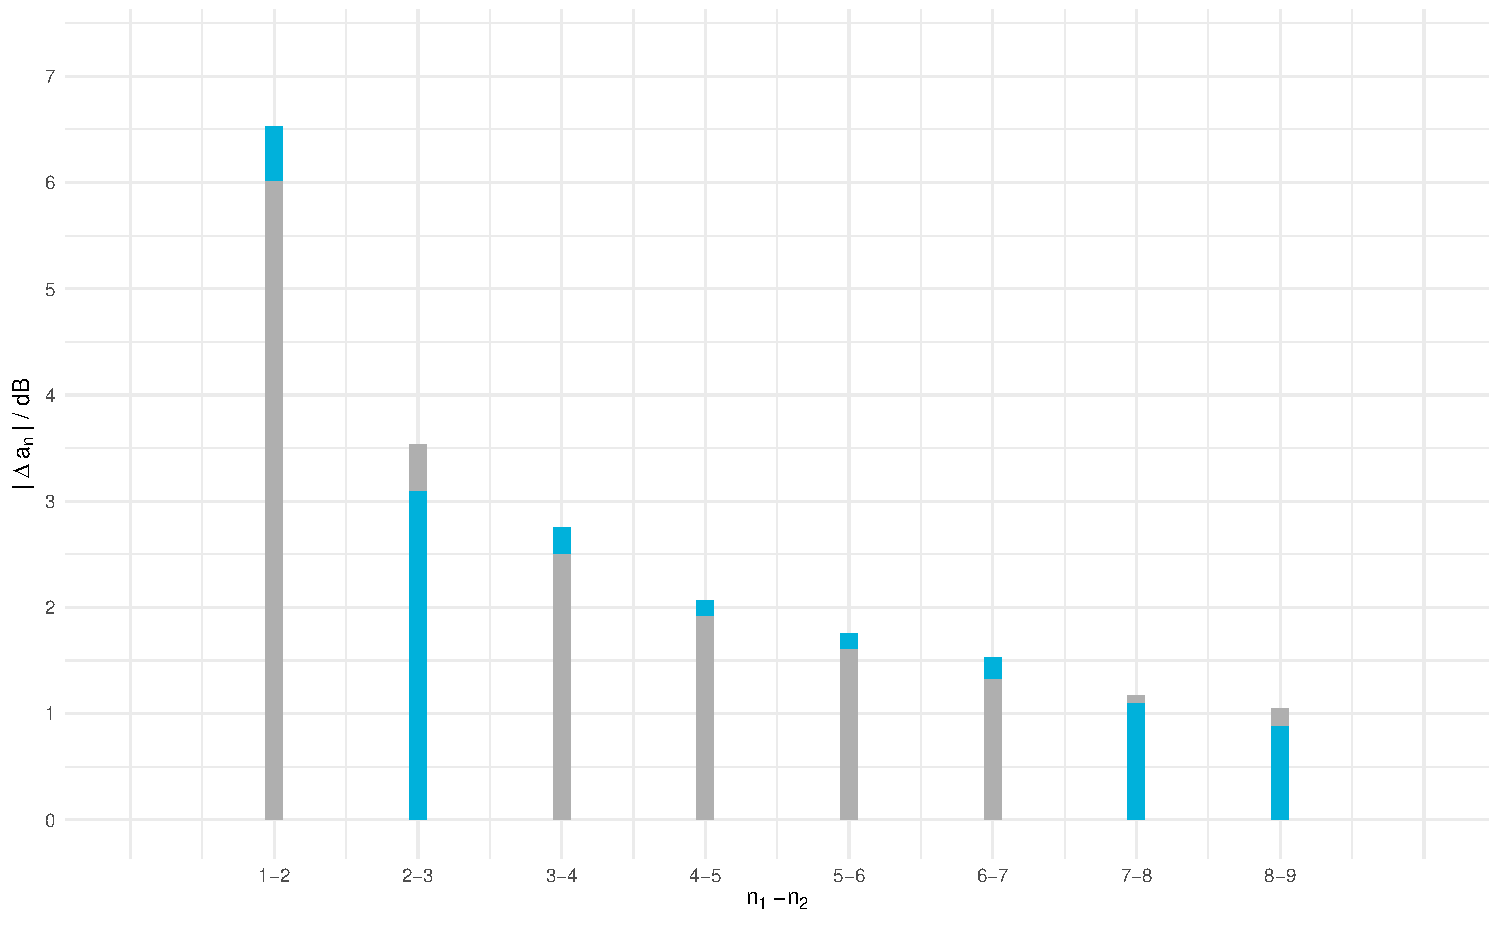
\includegraphics[width=\textwidth]{2_4/2_4_Amplivergleich}
  \caption{Vergleich der theoretischen (grau) und gemessenen (blau) Werte }
\end{figure}


\end{document}
